%\documentclass[a4paper,10pt]{jarticle}
%\documentclass[]{jarticle}
\documentclass[uplatex,10pt]{jsarticle}

%\usepackage{graphicx}
\usepackage[dvipdfmx]{graphicx}
\usepackage{eclbkbox} %breakbox用
\usepackage[T1]{fontenc}
\usepackage{lmodern}
\usepackage{amsmath}
\usepackage{here}
\usepackage{listings}

%本文領域を広め(空白箇所マージン領域を小さめ)に設定
\setlength{\textwidth}{179mm}
\setlength{\textheight}{251mm}
\setlength{\topmargin}{-2cm}
\setlength{\oddsidemargin}{-1cm}
\setlength{\evensidemargin}{-1cm}

\begin{document}

\title{情報工学実験IIレポート(探索アルゴリズム1)}
\author{曜日&グループ番号: 金曜日&グループ9} %
\date{実施日:2017年1月20日 (金)、提出日:2017年2月0日}

\maketitle


\section*{グループメンバ}
今回の実験はグループメンバ全員で取り組んだが,レポート化にあたって分担を行った.
グループメンバと担当した分野は次の通りである.
\begin{itemize}
 \item 155706J 久場翔悟: 担当Level2.1
 \item 155711E 平木宏空: 担当Level1.1,1.2,1.3
 \item 155716F 石塚海斗: 担当Level2.2
 \item 155730B 清水隆博: 担当Level2,Level2.3
\end{itemize}

\section*{提出したレポート一式について}
レポート一式は
``\verb|shell:/net/home/teacher/tnal/2016-search1-mon/group0/|''
にアップロードした。
提出したファイルのディレクトリ構成は以下の通りである。

\vspace{+0.5cm}
\begin{breakbox}
\begin{verbatim}
./src/      # 作成したプログラム一式
./report/   # レポート関係ファイル.図ファイルを含む.
./steepestsearch2-1/ #Level2.1で作成したプログラム一式
\end{verbatim}
\end{breakbox}

\newpage

\section{Leve l1: 最適化とは}
\subsection{Level 1.1: コンピュータと人間の違いを述べよ}
\subsubsection{課題説明}
コンピュータが人間より得意とするモノ、その反対に人間より不得手のモノ、両者について2つ以上の視点(立場や観点など)を示し、考察する。

\subsubsection{考察}
\begin{itemize}
 \item 視点1: hoge\\
コンピュータならば**が可能であり云々
 \item 視点2: fuga\\
人間は**しなくてはならないため云々
\end{itemize}

\subsection{Level 1.2: 住宅価格を推定するモデルについて}
\subsubsection{課題説明}
Housing Data Set\cite{housingdata}
におけるRM(平均部屋数)からMEDV(平均価格)を推定するた
めのモデルについて検討した。

\subsubsection{モデルへの入力}
\subsubsection{モデルにおける処理内容}
\subsubsection{モデルの出力}


(補足:PDF図を挿入する例)



\subsection{Level 1.3: モデルの良さを評価する方法について}
\subsubsection{課題説明}
Level 1.2 で検討したモデルの適切さを評価する指標について検討した。

\subsubsection{評価に用いる情報源}
\subsubsection{評価手順}
\subsubsection{評価に基づいた適切さを計る方法}



\newpage

\section{Level 2: 最急降下法による最適化}
\subsection{課題説明}
3種類の連続関数$y=x^2$、$z=x^2+y^2$、$y=-x \times cos(x)$について、
最急降下法の適用を通して探索挙動を観察した。
以下ではまず共通部分である最急降下法の探索手続きについて、
フローチャートを用いて解説する。
その後、3種類の関数毎にプログラムの変更箇所、
観察意図観察方法、観察結果、考察について説明する。


\subsection{Level 2共通部分}
(補足:Level2.1, 2.2, 2.3 には共通する部分が多いため、
共通部分は独立して報告すると良いでしょう)

\subsubsection{探索の手続き(共通部分)}

\subsubsection{フローチャート(共通部分)}
(手続きとフローチャートはまとめて一つの節にしても構いません)

 %共通部分の結果及び考察
\subsection{Level2.1: $y=x^2$ について}
\subsubsection{プログラムソース(変更部分)}
steepest\_decent.cの一部を以下のように変更した
\begin{lstlisting}[basicstyle=\ttfamily\footnotesize, frame=single]
    /** 以下の式を編集して完成させよ(1) **/
    z = x*x;

    /** 以下の式を編集して完成させよ(2-1) **/
    z_dx = 2*x;
\end{lstlisting}
更に今のalphaの値が見やすいように以下の出力を追加した。
\begin{lstlisting}[basicstyle=\ttfamily\footnotesize, frame=single] 
     printf("alpha = %.2f\n",alpha);
\end{lstlisting}
\subsubsection{観察意図と観察方法}
刻み値をより小さくすると探索点がより細かく移動するため最適性は良くなるだろう。しかし,小さくしすぎると最適性は良いが探索回数が増えてしまい,効率性は悪くなるだろう。

上記のように予想してこれを検証するために,seed値を1に固定しalphaの値を変えることにより探索を行い,結果を観測する。
\subsubsection{実行結果}
alphaの値を0.1から0.1刻みに1まで実行した。以下に実行結果の一部を示す。
\begin{lstlisting}[basicstyle=\ttfamily\footnotesize, frame=single]
alpha = 0.10
~~~~
step 62 x -0.0000072277 y 5.1121064439 f(x,y) 0.0000000001 5.224013e-11
step 63 x -0.0000057822 y 5.1121064439 f(x,y) 0.0000000000 3.343369e-11
~~~~
step 74 x -0.0000004967 y 5.1121064439 f(x,y) 0.0000000000 2.466971e-13
FINISH 3 step 75 x and y were not updated.

alpha = 0.20
~~~~
step 27 x -0.0000075424 y 5.1121064439 f(x,y) 0.0000000001 5.688705e-11
step 28 x -0.0000045254 y 5.1121064439 f(x,y) 0.0000000000 2.047934e-11
~~~~
step 34 x -0.0000002111 y 5.1121064439 f(x,y) 0.0000000000 4.457906e-14
FINISH 3 step 35 x and y were not updated.

alpha = 0.40
~~~~
step 8 x -0.0000188653 y 5.1121064439 f(x,y) 0.0000000004 3.558982e-10
step 9 x -0.0000037731 y 5.1121064439 f(x,y) 0.0000000000 1.423593e-11
~~~~
step 12 x -0.0000000302 y 5.1121064439 f(x,y) 0.0000000000 9.110995e-16
FINISH 3 step 13 x and y were not updated.

alpha = 0.50
step 0 x -7.3692442371 y 5.1121064439 f(x,y) 54.3057606266 5.430576e+01
step 1 x 0.0000000000 y 5.1121064439 f(x,y) 0.0000000000 0.000000e+00
FINISH 3 step 2 x and y were not updated.

alpha = 0.60
~~~~
step 8 x -0.0000188653 y 5.1121064439 f(x,y) 0.0000000004 3.558982e-10
step 9 x 0.0000037731 y 5.1121064439 f(x,y) 0.0000000000 1.423593e-11
~~~~
step 12 x -0.0000000302 y 5.1121064439 f(x,y) 0.0000000000 9.110995e-16
FINISH 3 step 13 x and y were not updated.

alpha = 0.90
~~~~
step 62 x -0.0000072277 y 5.1121064439 f(x,y) 0.0000000001 5.224013e-11
step 63 x 0.0000057822 y 5.1121064439 f(x,y) 0.0000000000 3.343369e-11
~~~~
step 84 x -0.0000000533 y 5.1121064439 f(x,y) 0.0000000000 2.844223e-15
FINISH 3 step 85 x and y were not updated.

alpha = 1.00
FINISH 1 step 1000 this trial couldn't be search enough under the term_cond=1000.
\end{lstlisting}

alphaの値が0.1のときから徐々にstep数が減少していき,alpha=0.5で最もstep数が少なくなった。更にalphaの値を増やしていくとstep数が増加していった。
\subsubsection{考察}
各alpha値でf(x)の値が0になる箇所を示したが,f(x)の表示されている範囲の値が0になってから実行が終わるまでにかかったstep数がalpha=0.5から離れるに連れて多くなっていることがわかった。偏微分の値がほぼ0になるとxの値が0に近づいているということになるが,そこから実行されている回数が多いほど更に細かく見ているため最適性が良くなると思った。しかし最も最適性がよかったalpha値から少なくなるごとに最適性が悪くなっていき,alpha値が低くても最適性が良いというわけではなかった。しかし効率性に関しては予想通り悪くなっていた(下図\ref{fig:alpha0.2},\ref{fig:alpha0.4},\ref{fig:alpha0.5})。

逆にalpha値が大きくなっていくと探索回数が増えていき,alpha=1.0からは実行が1000回を超えてしまった(下図\ref{fig:alpha1.0})。

探索点の推移のグラフから,alpha=0.2の際はほぼ0になってそこから動くことが少なくなった時点で動作を終了しているが,alpha=0.5の際は運が良く一度の試行で最小値を導いていることがわかる(下図\ref{fig:move_alpha0.2},\ref{fig:move_alpha0.5})。

alphaの値が小さくなりすぎると効率性に欠けてしまい,alphaの値が大きすぎると探索点が範囲外に出てしまう可能性が高くなってしまうことより,関数$y=x^2$に関して学習係数alphaは0より大きく1未満である適切な数が好ましいと考察される。今回seed値1の場合はalpha=0.5であった。

\begin{figure}[h]
 \begin{center}
  \begin{tabular}{c}
    \begin{minipage}{0.33\hsize}
    \begin{center}
    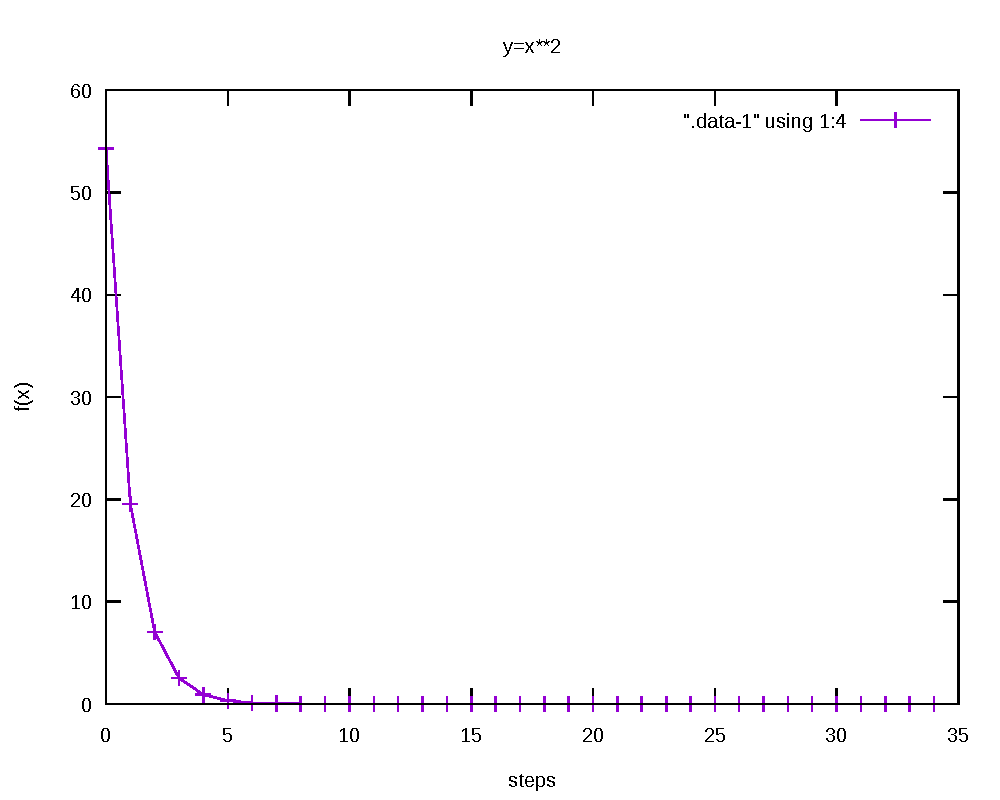
\includegraphics[width=5.0cm]{figs/alpha02.pdf}
    \caption{alpha=0.2での目的関数の推移}
    \label{fig:alpha0.2}
    \end{center}
    \end{minipage}
    
    \begin{minipage}{0.33\hsize}
    \begin{center}
    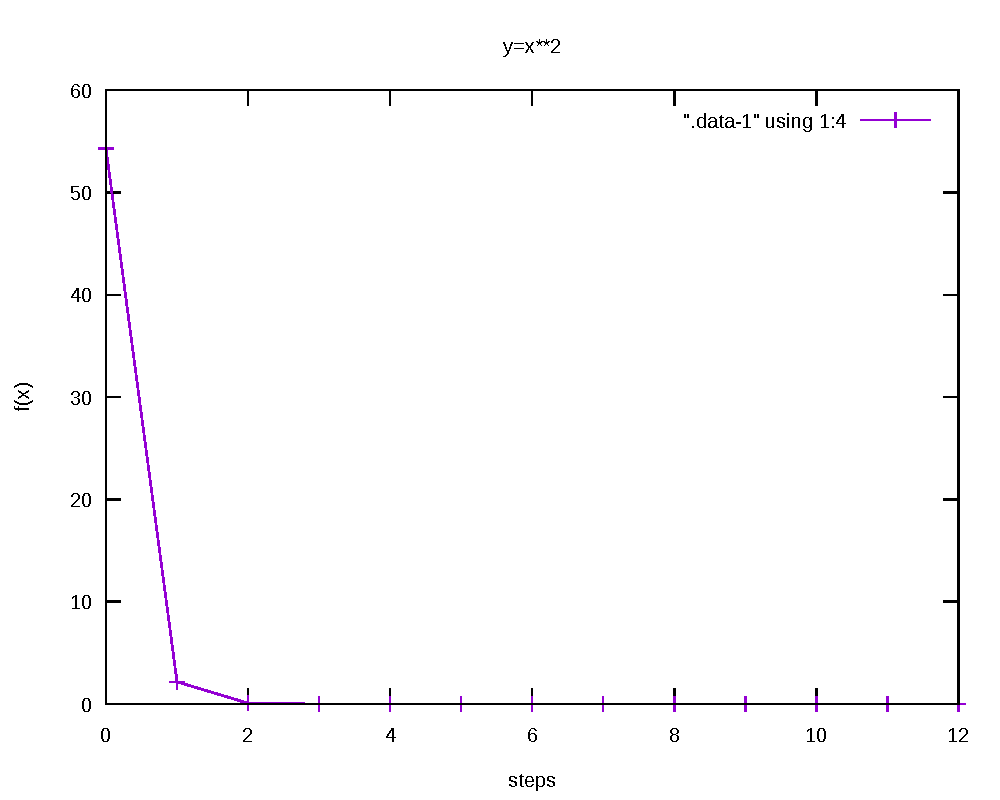
\includegraphics[width=5.0cm]{figs/alpha04.pdf}
    \caption{alpha=0.4での目的関数の推移}
    \label{fig:alpha0.4}
    \end{center}
    \end{minipage}
    
    \begin{minipage}{0.33\hsize}
    \begin{center}
    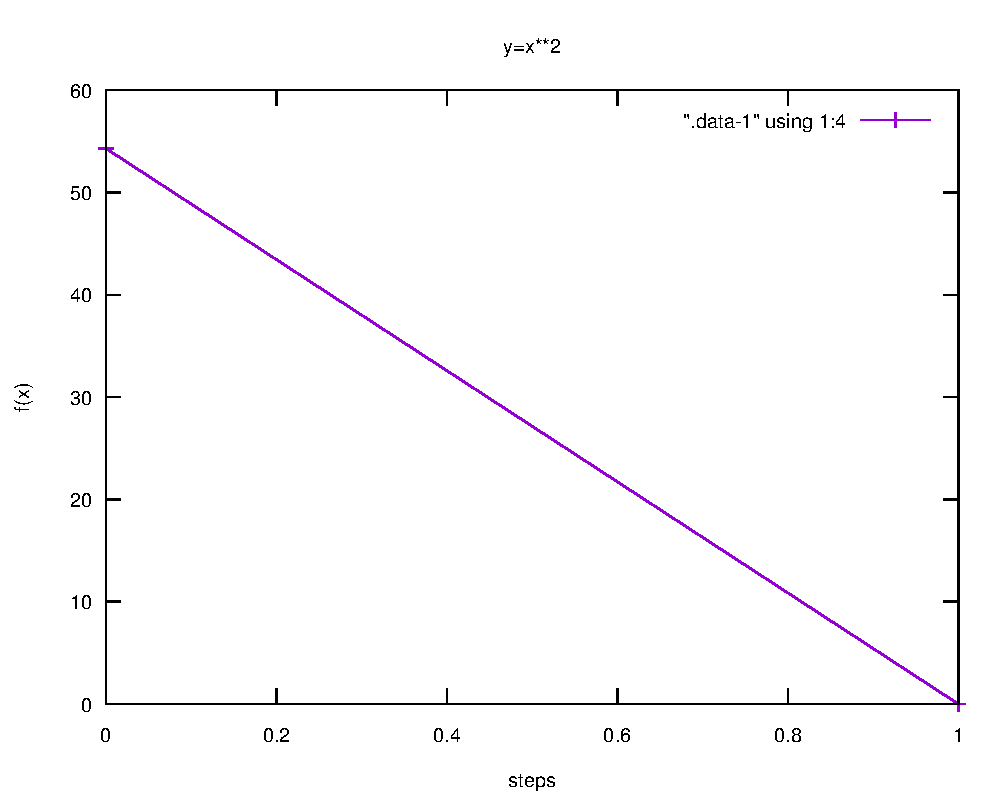
\includegraphics[width=5.0cm]{figs/alpha05.pdf}
    \caption{alpha=0.5での目的関数の推移}
    \label{fig:alpha0.5}
    \end{center}
    \end{minipage}
  \end{tabular}
 \end{center}
\end{figure}

\begin{figure}[h]
 \begin{center}
  \begin{tabular}{c}
    \begin{minipage}{0.33\hsize}
    \begin{center}
    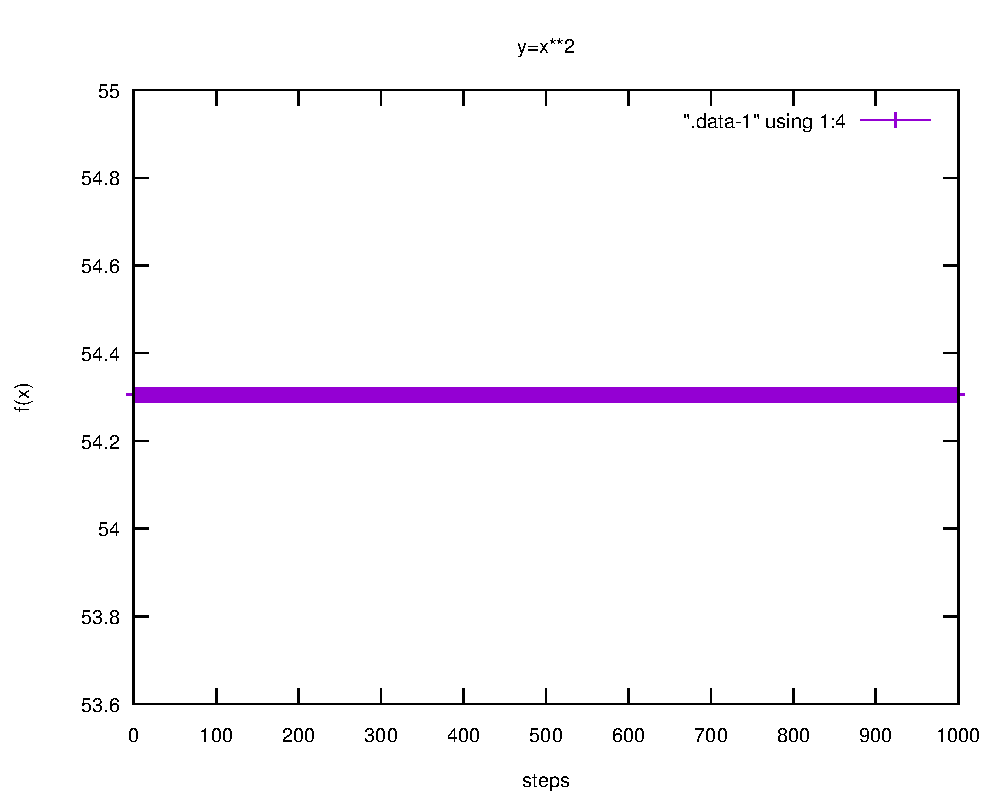
\includegraphics[width=5.0cm]{figs/alpha1.pdf}
    \caption{alpha=1.0での目的関数の推移}
    \label{fig:alpha1.0}
    \end{center}
    \end{minipage}
    
    \begin{minipage}{0.33\hsize}
    \begin{center}
    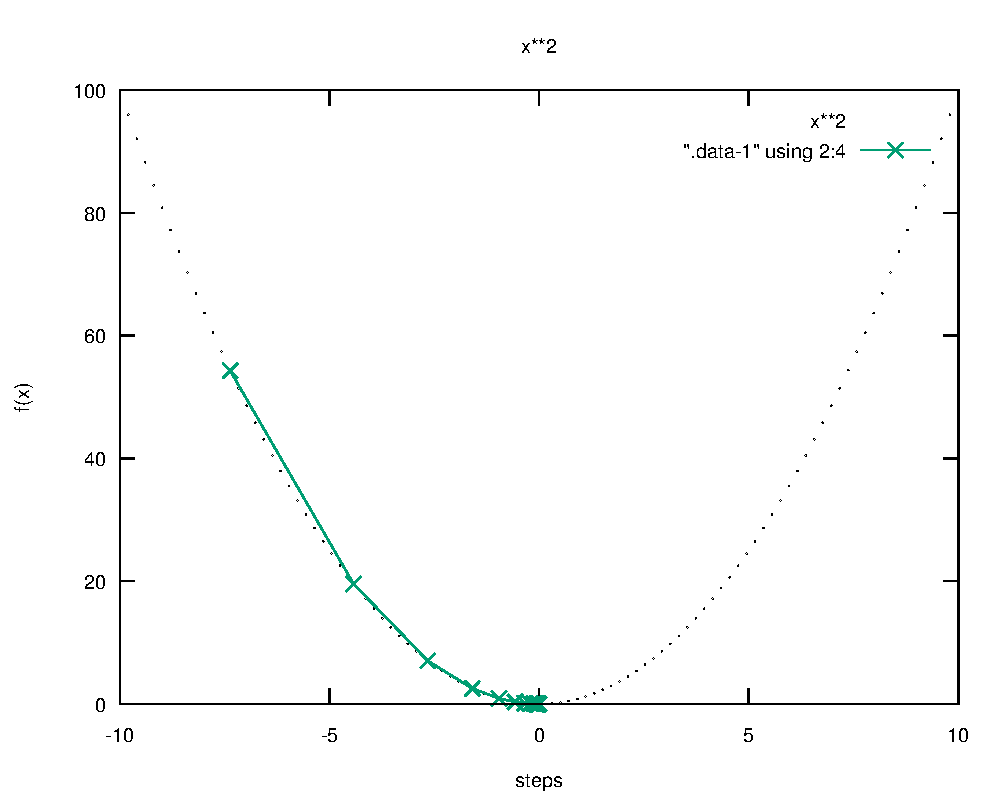
\includegraphics[width=5.0cm]{figs/move_alpha02.pdf}
    \caption{alpha=0.2での探索点の推移}
    \label{fig:move_alpha0.2}
    \end{center}
    \end{minipage}
    
    \begin{minipage}{0.33\hsize}
    \begin{center}
    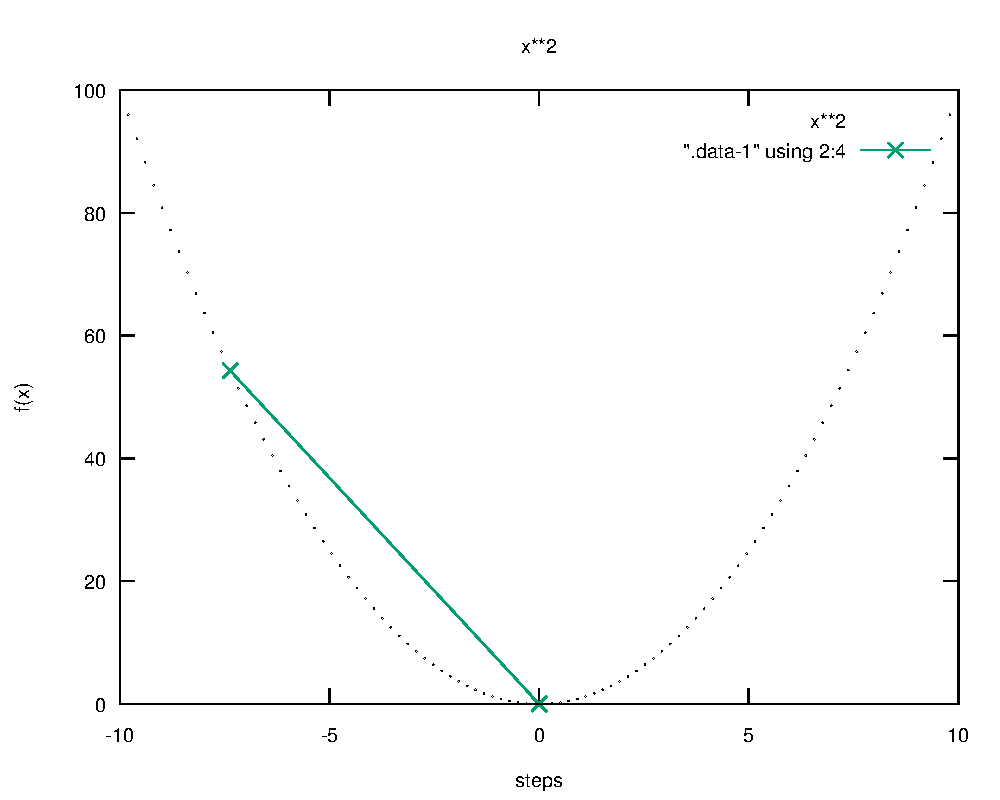
\includegraphics[width=5.0cm]{figs/move_alpha05.pdf}
    \caption{alpha=0.5での探索点の推移}
    \label{fig:move_alpha0.5}
    \end{center}
    \end{minipage}
  \end{tabular}
 \end{center}
\end{figure}
\subsection{Level2.2: $z=x^2 + y^2$ について}
\subsubsection{フローチャート共通からの変更点}
今回,Level2.2 に取り組むにあたって,プログラムの変更を行ったため,
フローチャートにも多少の変更が出た。\\
変更点を以下の図\ref{flow2.2}に示す。\\
  \begin{figure}[H]
	\begin{center} %センタリングする
	  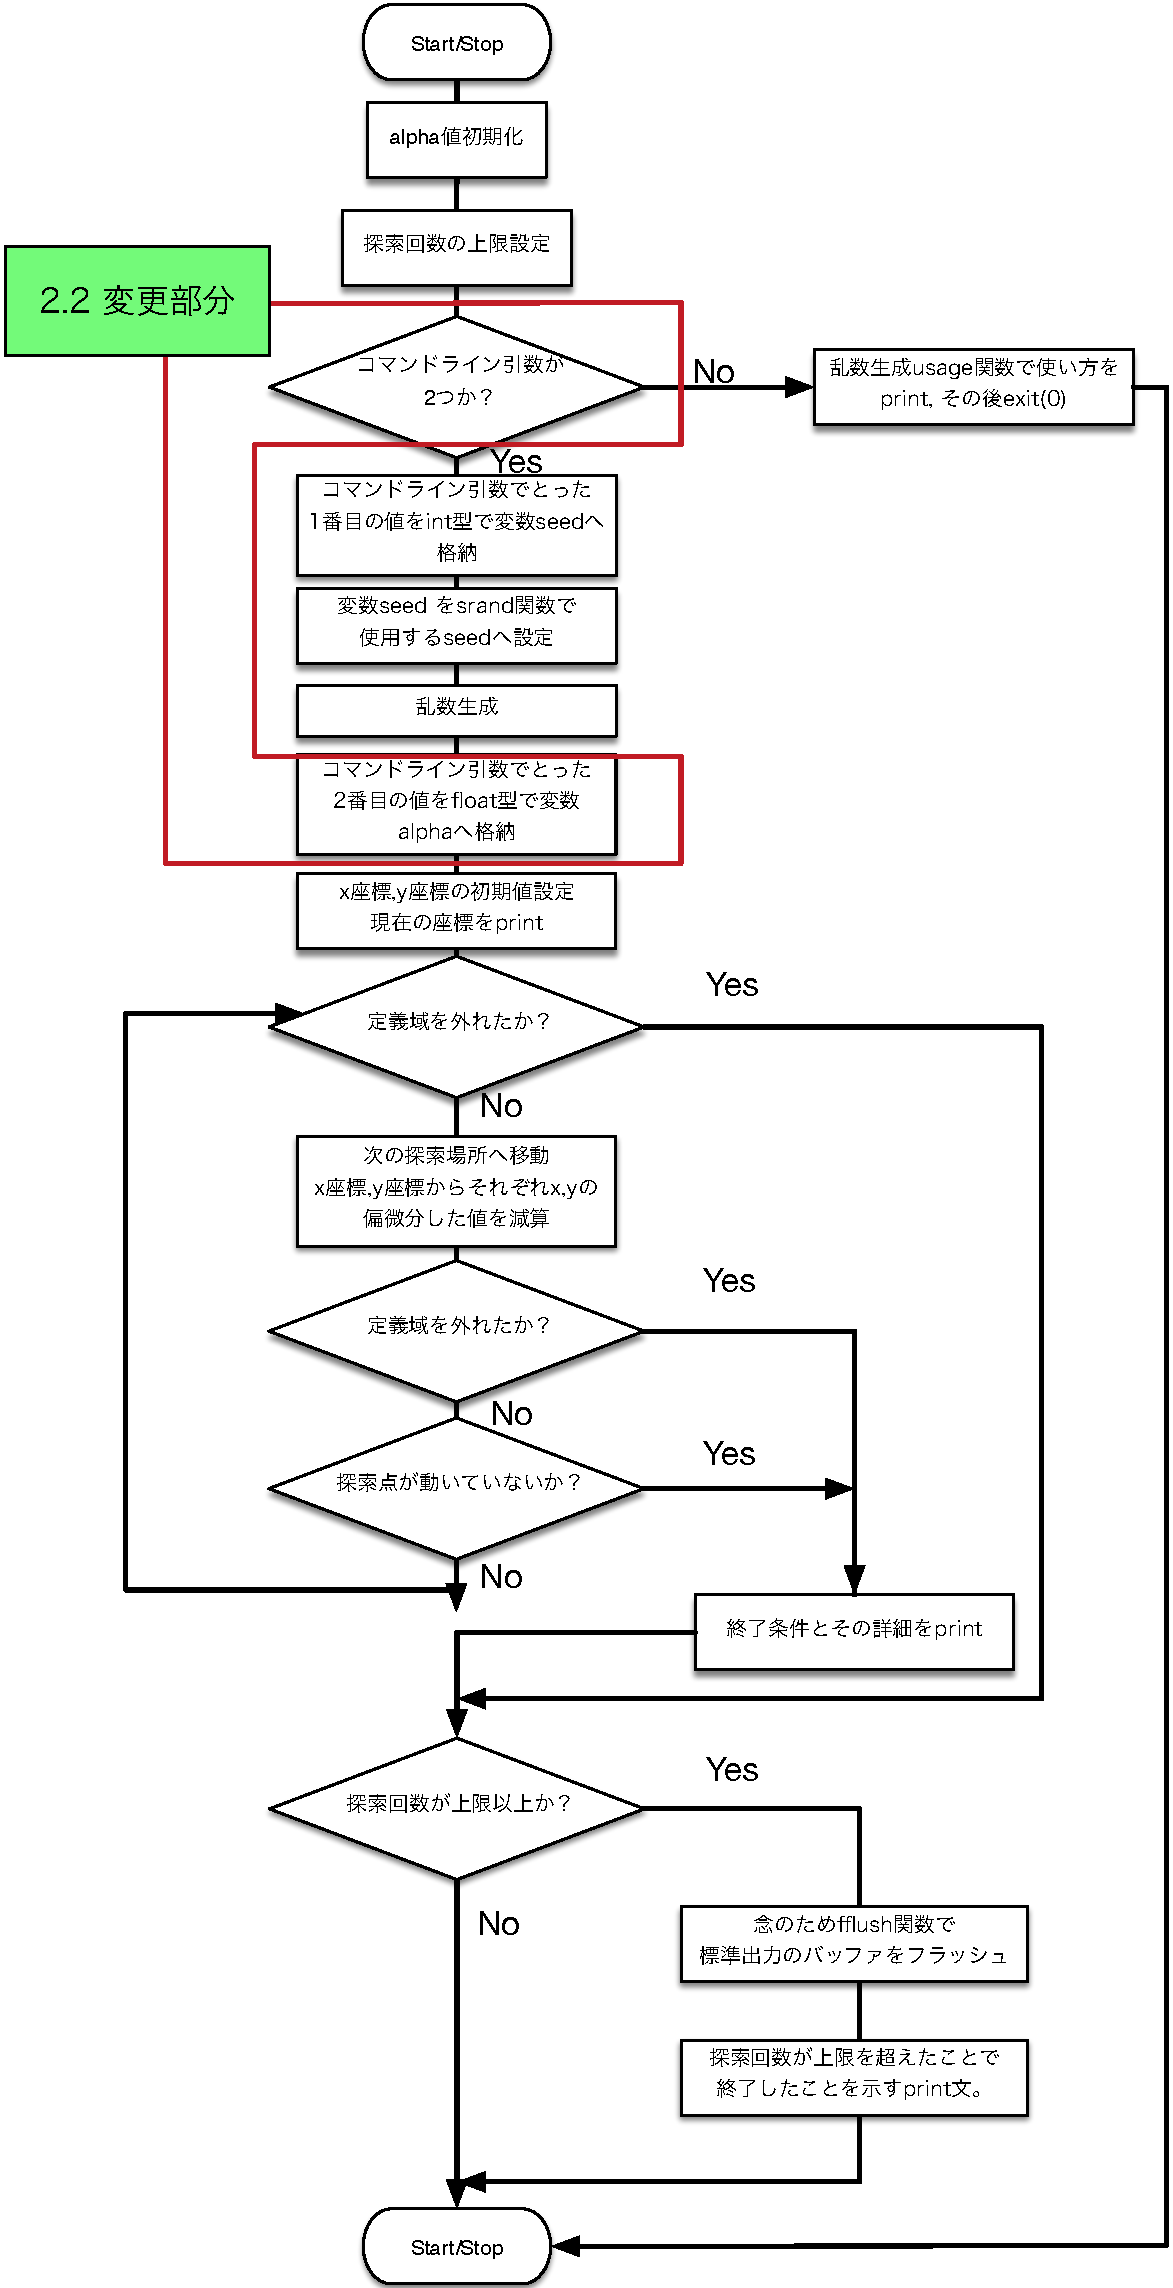
\includegraphics[scale=0.45]{./flowchart2-2.pdf}
	  \caption{フローチャート変更点} %タイトルをつける
	  \label{flow2.2} %ラベルをつけ図の参照を可能にする
	\end{center}
  \end{figure}


\subsubsection{プログラムソース(変更部分)}
以下の図\ref{cp22}に変更部分のみを示す。
	\begin{figure}[H]
        \caption{Level2.2 変更点}
		\label{cp22}
		\fontsize{10pt}{10pt}\selectfont
      	\begin{shadebox}
        	\begin{verbatim}
			//main 関数直後
			f( argc != 3 ){
			(略)
			}else{
			(略)
			alpha = atof(argv[2]); 
			(略)
			}
			
			//f 関数内
			//  z = x;
			  z = x*x + y*y;

			//pd_x 関数内
			//  z_dx = 1;
			  z_dx = 2*x;

			//pd_y 関数内
			//  z_dy = 0;
			  z_dy = 2*y;
        	\end{verbatim}
      	\end{shadebox}
     \end{figure}

\subsubsection{観察意図と観察方法}
seed値を固定してalpha 値を変動させることで,探索点の刻み幅による探索の最適性及び
効率性を検討する。
alpha 値を変更することで探索幅も変動することから,以下の2つのような予想が立てられる。
1, alpha 値が大きければ探索点の刻み幅も大きくなり,効率性を向上できるが,最適性が低下
する。
2, alpha 値が小さければ探索点の刻み幅が小さくなるため,最適性を向上できるが,効率性
が低下する。\\
効率性の観察方法は,seed値を固定しalpha 値を変動させた際のstep 数の推移を
各seed 値(範囲1000-10000 1000刻み)ごとに表して行う。
効率性の検討はグラフより,各seed 数で最小step 数のalpha 値を読み取り,
最も優れたalpha 値を多数決で決定し,それをこのプログラムの最大効率であると決定,
改善点を考察する。\\
また,srand 関数にコマンドライン引数のseed 値が渡されているため,
rand 値は同じseed 値 を入力している限り,一定である。よって,同一seed 値 において,
乱数を考慮しての複数実行,実行結果の平均値取得等はしない。\\
最適性の観察方法は,seed値を固定しalpha 値を変動させた際の終了時座標,これと
傾きが0になっている座標(ここでは0,0)との差の推移を各seed 値
(範囲1000-10000 1000刻み)ごとにグラフで表す。
最適性の検討はグラフからその差が最小のalpha の値を各seedから読み,最も優れた
alpha 値を多数決で決定する。
そのalpha 値をこのプログラムの最大最適値 であると決定し,改善点を考察する。

\subsubsection{実行結果}
  \begin{enumerate}
  \renewcommand{\labelenumi}{\arabic{enumi}}

  \item 効率性について\\
	効率性の観察のための手法として,各seed値(1000-10000の1000刻み10種),
	各alpha値(0.001 と 0.1-1.0(0.1刻み)の計11種) ごとに
	最終step数をplot していき,その推移傾向を観察することで行った。\\
	以下の図\ref{stepgraph1}がその結果である。

  \begin{figure}[H]
	\begin{center} %センタリングする
	  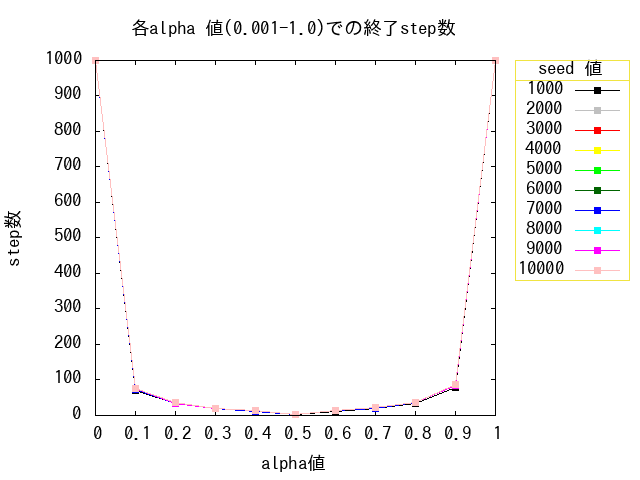
\includegraphics[width=9cm]{../steepestsearch2-2/createStepGraph/StepGraph.png}
	  \caption{各alpha値(0.001-1.0) での終了step数} %タイトルをつける
	  \label{stepgraph1} %ラベルをつけ図の参照を可能にする
	\end{center}
  \end{figure}

  alpha 値が 0.001, 1.0 の時に step数が1000となり,alpha 値 0.1-0.9 までの
  点の差が見えづらい。よって,alpha 値が0.1-0.9 の範囲の最終step数のグラフも
  図\ref{stepgraph2}に用意した。
  \begin{figure}[H]
	\begin{center} %センタリングする
	  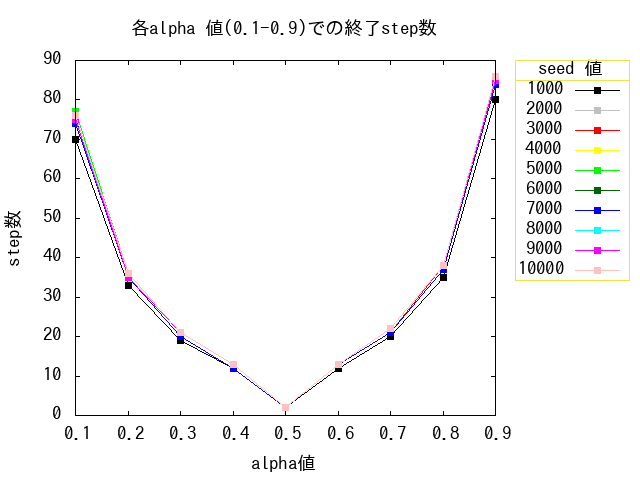
\includegraphics[width=9cm]{../steepestsearch2-2/createStepGraph/StepGraph2.png}
	  \caption{各alpha値(0.1-0.9) での終了step数} %タイトルをつける
	  \label{stepgraph2} %ラベルをつけ図の参照を可能にする
	\end{center}
  \end{figure}


  \item 最適性について\\
	最適性の観察のための手法として,各seed値(1000-10000の1000刻み10種),
	各alpha値(0.001 と 0.1-1.0(0.1刻み)の計11種) ごとに
	終了座標の誤差(x,yの合計)をplot していき,その推移傾向を観察することで行った。\\
	以下の図\ref{diffgraph1}がその結果である。


  \begin{figure}[H]
	\begin{center} %センタリングする
	  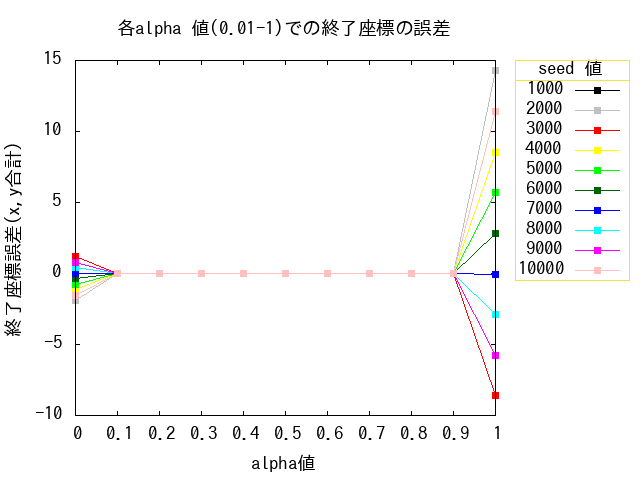
\includegraphics[width=9cm]{../steepestsearch2-2/createDiffGraph/DiffGraph.png}
	  \caption{各alpha値(0.001-1.0) での終了座標誤差(x,y合計)} %タイトルをつける
	  \label{diffgraph1} %ラベルをつけ図の参照を可能にする
	\end{center}
  \end{figure}

  alpha 値が 0.001, 1.0 の時に 最大合計誤差10を超え,alpha 値 0.1-0.9 までの
  点の差が見えづらい。よって,alpha 値が0.1-0.9 の範囲の合計誤差のグラフも
  図\ref{stepgraph2}に用意した。
  \begin{figure}[H]
	\begin{center} %センタリングする
	  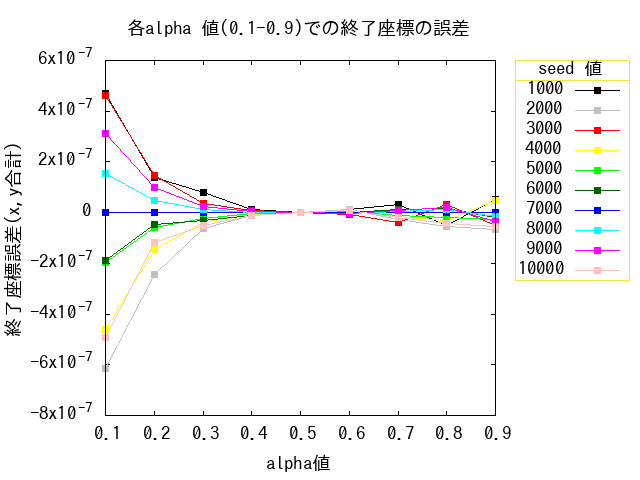
\includegraphics[width=9cm]{../steepestsearch2-2/createDiffGraph/DiffGraph2.png}
	  \caption{各alpha値(0.1-0.9) での終了座標誤差(x,y合計)} %タイトルをつける
	  \label{diffgraph2} %ラベルをつけ図の参照を可能にする
	\end{center}
  \end{figure}

  \end{enumerate}

\subsubsection{考察}
まず,効率性についての考察を行う。\\
図\ref{stepgraph1}より,最終step数が1000回以内に収まるのが,$0.001 < alpha < 1.0$
の範囲であることがわかる。このことから,alpha 値が小さすぎると探索できる
範囲が狭まり,最適解まで届かなかったと推察する。 図\ref{stepgraph2}からは,
総step数が1番低い点のalpha 値が 0.5 であり,0.5 から離れるごとにstep 数が
増加する傾向にあることがわかる。alpha値が0.5 の時に総step数が最小となった理由を,
プログラム内の探索点移動に用いられている式より考察する。\\
$x = x - alpha*pd_x(x,y);$\\
この式のpd\_x(x,y) はxについての偏微分であるため,置き換えると\\
$x = x - alpha*2x;$\\
となる。この式に alpha = 0.5 を代入すると x には '0' が入ることとなるため,
移動後のx座標がちょうど傾きが0になる点(最終的に移動したい最適解)になる。
yについても同様にしてalpha = 0.5 の時に1回移動後の座標は'0'となる。\\
このことから, alpha = 0.5 という値は 今回探索した $x^2 + y^2$ の式において
あらゆる座標から最適解の座標を求めることができる値であることがわかる。\\

次に,最適性について\\
効率性の考察にて
図\ref{stepgraph1}より,最終step数が1000回となるのが$alpha=0.001 , alpha=1.0$
で,言い換えると$alpha=0.001 , alpha=1.0$のとき最適解との誤差が大きい。\\
このことが,終了座標誤差を表す図\ref{diffgraph1}からも読み取れる。
図\ref{diffgraph2}からは効率性と同じく alpha=0.5 に最適性が最も高いことがわかる。
さらにalpha=0.5 の点へのグラフの収束の度合いにも alpha が0.5より小さい時と
大きい時で差がある。これは,alphaが0.5より小さい場合の最適解からの誤差は探索点が
単純に最適解に届かなかったものであるが,alpha が0.5より大きい場合では
最適解付近まで探索点が到達したが探索点の移動幅の大きさが影響し最適解には
至らなかったというもの,という差によるものと推察する。


\subsection{Level2.3: $y=-x*cos(x)$ について}
\subsubsection{プログラムソース(変更部分)}
\subsubsection{観察意図と観察方法}
\subsubsection{実行結果}
\subsubsection{考察}



\vspace{+1.0cm}
(補足:参考文献は thebibliography 環境を使って列挙し、
本文中で適切な箇所で引用するようにしましょう。
例えば下記文献は、アブストラクトやLevel 4で引用しています)
\begin{thebibliography}{99}
\bibitem{info2-search1}
情報工学実験2: 探索アルゴリズムその1(當間)\\
\verb|http://www.eva.ie.u-ryukyu.ac.jp/~tnal/2016/info2/search1/|
\bibitem{housingdata}
Housing Data Set\\
\verb|http://archive.ics.uci.edu/ml/datasets/Housing|
\end{thebibliography}

\end{document}
